\documentclass{article}

\usepackage{amsmath}
\usepackage[margin=1in]{geometry}
\usepackage{listings}
\usepackage{hyperref}
\usepackage{graphicx}
\usepackage{amssymb}
\usepackage{verbatim}
\usepackage{siunitx}
\usepackage{enumitem}
\usepackage{bbm}
\usepackage{bm}
\usepackage{caption}
\usepackage{algpseudocode}
\usepackage{algorithm}
\usepackage[square,sort,comma,numbers]{natbib}

\newcommand{\norm}[1]{\left\lVert#1\right\rVert}
\newcommand{\normtwo}[1]{\left\lVert#1\right\rVert_2}
\newcommand{\abs}[1]{\left\lvert#1\right\rvert}
\newcommand{\mat}[1]{\bm{{#1}}}
\renewcommand{\vec}[1]{\bm{{#1}}}
\newcommand{\lequiv}{\Leftrightarrow}
\newcommand{\bigO}[1]{\mathcal{O}\!\left(#1\right)}
\newcommand{\ceil}[1]{\left\lceil #1 \right\rceil}
\newcommand{\floor}[1]{\left\lfloor #1 \right\rfloor}
\newcommand{\sfrac}[2]{#1/#2}
\newcommand{\hquad}{\enskip}
\newcommand{\expected}[1]{\mathbb{E}\left[#1\right]}
\newcommand{\mspan}[1]{\text{span}\left( #1 \right)}
\newcommand{\prob}[1]{P\left(#1\right)}
\newcommand{\probt}[1]{P\left( \text{#1} \right)}
\newcommand{\condprob}[2]{P\left(#1 \:|\: #2\right)}
\newcommand{\condprobt}[2]{P\left(\text{#1} \:|\: \text{#2}\right)}
\newcommand{\bayes}[2]{\frac{\condprob{#2}{#1}\prob{#1}}{\prob{#2}}}
\newcommand{\bayesx}[3]{\frac{\condprob{#2}{#1}\prob{#1}}{\condprob{#2}{#1}\prob{#1} + \condprob{#2}{#3}\prob{#3}}}
\newcommand{\sech}{\text{sech}}
\newcommand*{\qed}{\hfill\ensuremath{\blacksquare}}%
\newcommand*{\vertbar}{\rule[-1ex]{0.5pt}{2.5ex}}
\newcommand*{\horzbar}{\rule[.5ex]{2.5ex}{0.5pt}}
\newcommand{\vect}[2]{\underline{{#1}}_{{#2}}}
\newcommand{\basisp}[1]{\underline{{p}}_{{#1}}}
\newcommand{\basisq}[1]{\underline{{q}}_{{#1}}}
\newcommand{\coeff}[1]{\underline{{a}}_{{#1}}}
\newcommand{\bestfit}{\underline{\bar{x}}}
\newcommand{\grad}{\nabla}
\newcommand{\laplace}{\Delta}


\begin{document}
\section{Background}
The problem being solved is the Poisson problem in one dimension:
$$ \grad^2\vec{u} = -f $$
$$ f(\vec{x}) = \vec{x} $$
Defined on the following domain with Dirichlet boundary conditions:
$$ \Omega = \left[-1, 1\right]$$
$$ \partial\Omega = 0 $$
This is discretized using finite differences on a grid of $N=31$ equispaced points and results in the following system:
$$ \mat{A}\vec{u} = \vec{x} $$
where
$$\mat{A} = \frac{1}{h^2} \text{tridiag}\left(\left[-1, 2, -1\right]\right)$$
$$h = \frac{1}{N+1}$$

The above linear system is solved using a two-level V cycle multigrid method using the following steps:

\begin{enumerate}
\item Generate an initial random guess, $\vec{u}_0$.
\item Pre-smooth the guess using one iteration of Jacobi using weight $\omega$.
\item Restrict the grid and residual using the operator $\mat{R}=\mat{P}^T$.  The given interpolation operator $\mat{P}$ is constructed as the \textit{ideal interpolation operator}.
\item Perform a linear solve on the restricted residual to obtain the coarse solution.
\item Interpolate the solution to the fine grid using operator $\mat{P}$.
\item Post-smooth using one iteration of Jacobi, with same weight $\omega$.
\end{enumerate}

The Jacobi smoothing weight that is used, $\omega$, is the optimal weight that minimizes the overall factor of convergence for the method:

$$\omega = \arg \min_{\omega\in\left(0,1\right)} \lim_{k\to\infty} \frac{ \vec{u}_{k+1} - \vec{u}^* }{ \vec{u}_{k} - \vec{u}^* }$$

where $\vec{u}^*$ is the ``optimal'' solution, precomputed by a dense linear solve.  Computationally, $\omega$ is approximated a bracked numerical optimization method, with the assumption that $\omega$ is unimodal with respect to the convergence factor.

\section{Generating Coarse Grids}

To train the model, a set of 96000 C/F grids were randomly generated via random perturbation.  Several ``reference'' grids were generated according to varying coarsening factors, of which the following values were used:

$$r = \left\{
\frac{1}{9},\quad
\frac{1}{8},\quad
\frac{1}{7},\quad
\frac{1}{6},\quad
\frac{1}{5},\quad
\frac{1}{4},\quad
\frac{1}{3},\quad
\frac{1}{2},\quad
2,\quad
3,\quad
4,\quad
5,\quad
6,\quad
7,\quad
8,\quad
9
\right\}$$

where values of $r<1$ refer to grids where every $\frac{1}{r}$ points is a fine point and the rest coarse, and $r>1$ refers to grids with every $r$ points being a coarse point and the rest fine.  These grids were then used to solve the Poisson problem and their weights and convergence factors recorded.

Each reference grid was randomly permuted such that each grid point had a random probability of being flipped to the opposite value.  I.e. coarse point to fine, and fine point to coarse.  Random trials of the following probabilities were used:

$$ p = \left\{0.01, \quad 0.05, \quad 0.1, \quad 0.25, \quad 0.5, \quad 0.75\right\} $$

For each value of $p$, $1000$ random grids were generated according to the above permutation strategy.  Each random grid was then also used to solve the defined Poisson problem, and the optimal Jacobi weight, $\omega$, and convergence factor were recorded.

In total, 16 convergence factors $\times$ 6 probability trials $\times$ 1000 random iterations = 96000 random grids were created.  The code used to generate these grids is given in \texttt{grids/gen\_grids.py}.

\section{CNN Model}

In an attempt to predict both optimal Jacobi weight and factor of convergence given an arbitrary grid, a CNN of the following architecture was trained\footnote{I neither claim that this CNN is optimal nor was its architecture particularly well thought-out.  I am sure that tweaking the layers will obtain better results}:

\begin{enumerate}
\item 1-dimensional convolutional layer with kernel size $7$.  Input 1 layer, output 20 layers.  ReLU activation function.
\item Max pooling layer with kernel size 2 and stride 2.  This takes the maximum element of each block of $2$ elements, and effectively cuts the size of the input tensor in half.
\item 1-dimensional convolutional layer with kernel size $5$.  Input 20 layers, output 20 layers.  ReLU activation function.
\item Max pooling layer with kernel size 2 and stride 2.
\item 1-dimensional convolutional layer with kernel size $3$.  Input 20 layers, output 20 layers.  ReLU activation function.
\item Max pooling layer with kernel size 2 and stride 2.
\item Fully connected layer with input size 20, output size 15.  ReLU activation function.
\item Fully connected layer with input size 15, output size 10.  ReLU activation function.
\item Fully connected layer with input size 10, output size 1.  ReLU activation function.
\end{enumerate}

\subsection{Training}

The previously generated set of 96000 random grids was split into training and testing sets, with a random $85\%$ of entries going to the training set and the remaining $15\%$ going into the testing set.

The grids were formed into a $N\times 1 \times n$ tensor, with $N=96000$ being the number of grids and $n=31$ being the grid size.  The tensor representation was formed by means of assigning $1$ to coarse points and $-1$ to fine points:

$$
T_{i1k} = \begin{cases}
1 & \text{point $k$ in grid $i$ is coarse}\\
-1 & \text{point $k$ in grid $i$ is fine}
\end{cases}
$$

Of course, this assignment is arbitrary and swapping the values would produce similar results.  The input weights were then normalized such that their range lies between $\left[0, 1\right]$.  When displaying any output from the CNN, this transformation must be undone for the results to be sensible.  The grid dataset class contains a \texttt{scale\_output()} method to do this in \texttt{jacobi-cnn/model.py}.

For the Jacobi model, the CNN was trained for 100 epochs while for the convergence factor model it was trained for 300 epochs.  Training was done using a MSE (mean-square error) loss function with stochastic gradient descent.  In each iteration, minibatches of size $500$ were used to train and backpropagate the model.  Since the number of training samples is not evenly divisible by $500$, these ``extra'' samples were arbitrarily discarded at each iteration.  The MSE loss and L1 loss at each iteration is given by Figures \ref{fig:jacobi_loss}, \ref{fig:conv_loss}.  These are also compared against the loss of a ``trivial predictor'', where the predicted value is simply the average of all input values.

\subsection{Results}

Results of plotting the true vs predicted Jacobi weights and convergence factors can be seen in Figures \ref{fig:jacobi_preds} and \ref{fig:conv_preds}, respectively.  Interesting ``peaks'' in the predicted values occur when the CNN is more optimistic than the actual Jacobi or convergence factor allows.  These results are interesting and the input grids could perhaps be extreme outliers.  The convergence factor values still have quite a large relative error, but the results seem to be encouraging and suggest that a convergence factor could actually be learned.  A grid corresponding to one of the dips is displayed in Figure \ref{fig:worst}.

As a fun experiment, the most ``convergent'' (or a local minimum) was found by numerically optimizing a random input tensor until the convergence factor was minimized.  Results of this can be seen in Figure \ref{fig:optimized_grid}.

\begin{figure}[h]
  \centering
  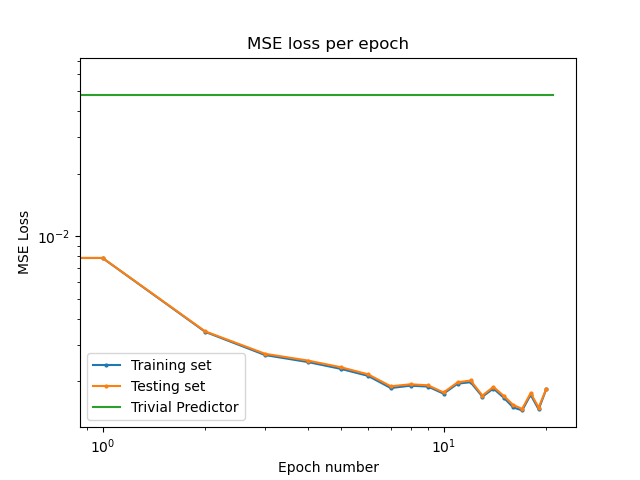
\includegraphics[scale=0.7]{figures/jacobi-conv/jacobi_mse.png}
  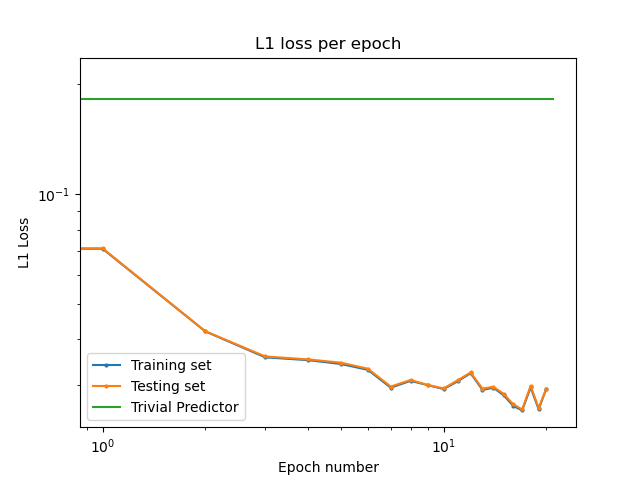
\includegraphics[scale=0.7]{figures/jacobi-conv/jacobi_l1.png}
  \caption{MSE, L1 loss per training iteration for Jacobi weights}
  \label{fig:jacobi_loss}
\end{figure}

\begin{figure}[h]
  \centering
  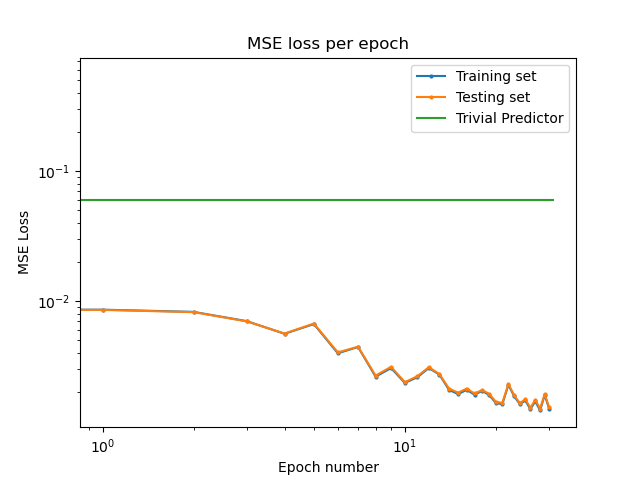
\includegraphics[scale=0.7]{figures/jacobi-conv/conv_mse.png}
  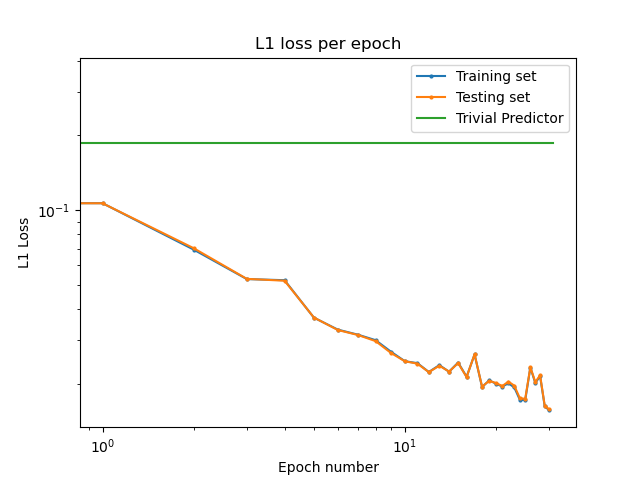
\includegraphics[scale=0.7]{figures/jacobi-conv/conv_l1.png}
  \caption{MSE, L1 loss per training iteration for convergence factor}
  \label{fig:conv_loss}
\end{figure}

\begin{figure}[h]
  \centering
  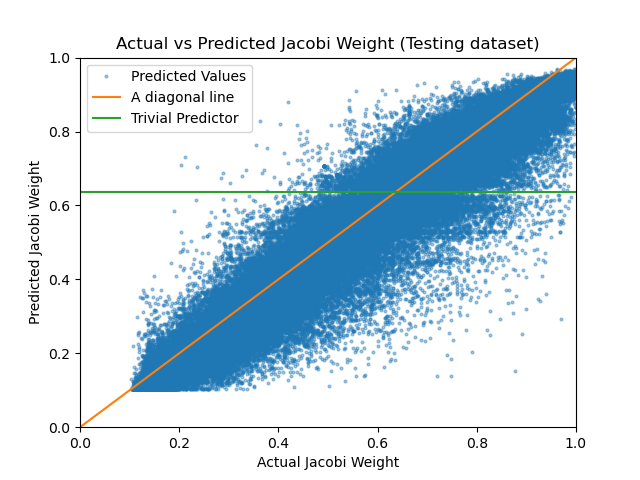
\includegraphics[scale=0.7]{figures/jacobi-conv/jacobi_test_pred.png}
  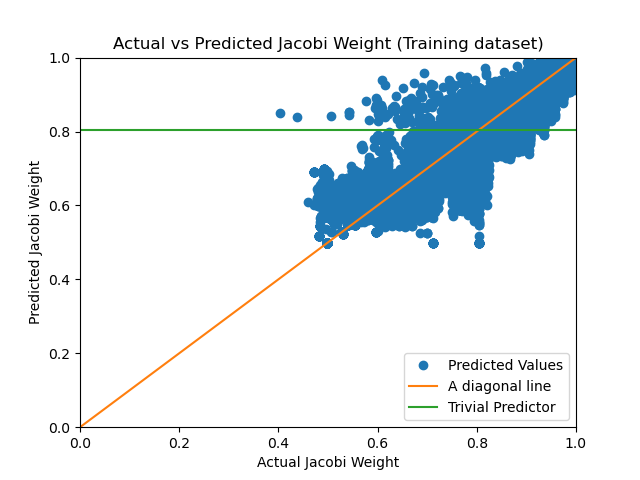
\includegraphics[scale=0.7]{figures/jacobi-conv/jacobi_train_pred.png}
  \caption{Predicted vs Actual Jacobi Weights}
  \label{fig:jacobi_preds}
\end{figure}

\begin{figure}[h]
  \centering
  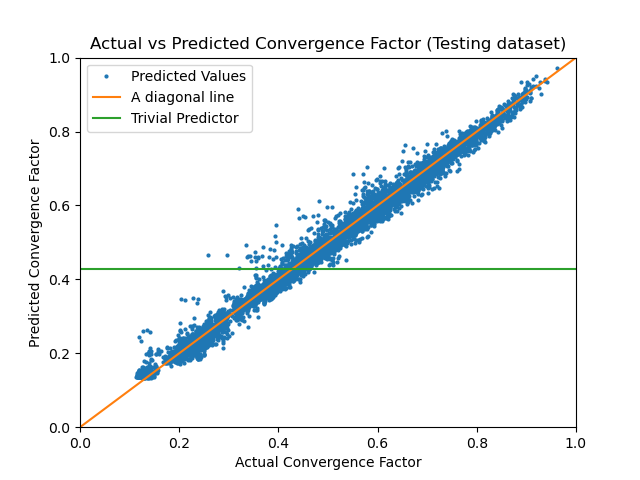
\includegraphics[scale=0.7]{figures/jacobi-conv/conv_test_pred.png}
  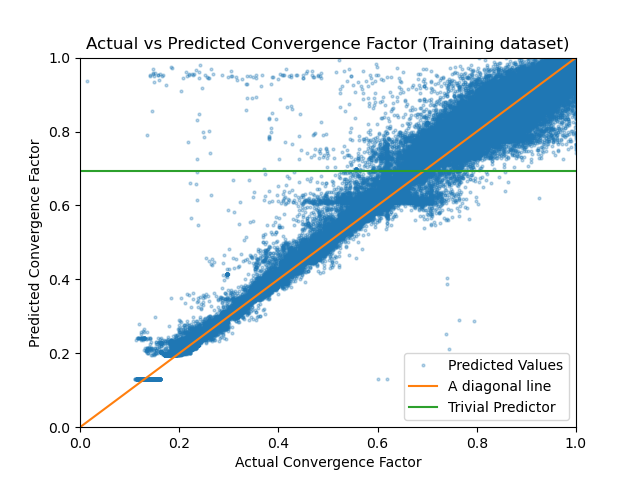
\includegraphics[scale=0.7]{figures/jacobi-conv/conv_train_pred.png}
  \caption{Predicted vs Actual Convergence Factors}
  \label{fig:conv_preds}
\end{figure}

\begin{figure}[h]
  \centering
  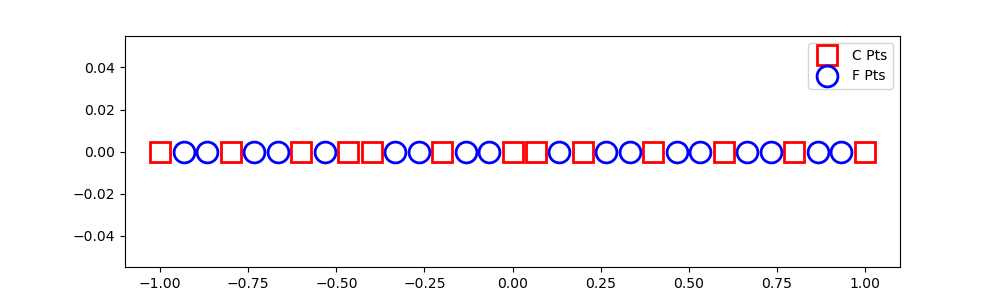
\includegraphics[scale=0.7]{figures/jacobi-conv/conv_peak_worst_err.png}
  \caption{Grid corresponding to worst prediction error.  Actual value of $\omega=0.6799$, predicted $\hat{\omega} = 0.2950$.  Absolute error $0.384$, relative error $0.566=56.6\%$.}
  \label{fig:worst}
\end{figure}

\begin{figure}[h]
  \centering
  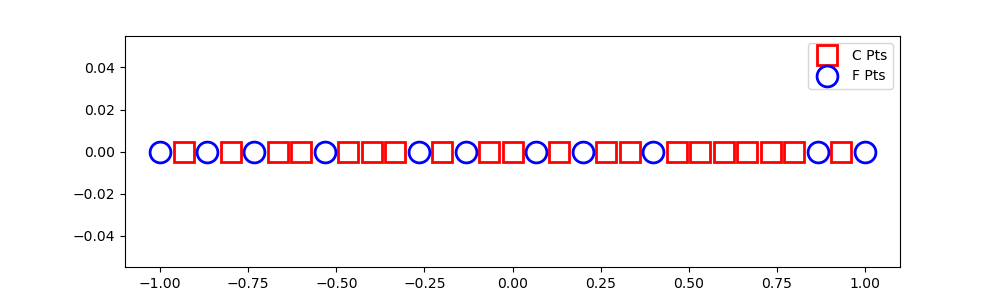
\includegraphics[scale=0.7]{figures/jacobi-conv/conv_opt_grid.png}
  \caption{Grid obtained by numerically optimizing CNN output.  The neural net was run ``in reverse'', by running SGD on the input tensor instead of the network weights.  Values $>0$ were interpreted as coarse points, and negative values as fine points.  True convergence factor: $0.2327$, predicted factor: $0.2179$.}
  \label{fig:optimized_grid}
\end{figure}

\end{document}
